\documentclass[oneside,numbers,spanish]{ezthesis}
%% # Opciones disponibles para el documento #
%%
%% Las opciones con un (*) son las opciones predeterminadas.
%%
%% Modo de compilar:
%%   draft            - borrador con marcas de fecha y sin im'agenes
%%   draftmarks       - borrador con marcas de fecha y con im'agenes
%%   final (*)        - version final de la tesis
%%
%% Tama'no de papel:
%%   letterpaper (*)  - tama'no carta (Am'erica)
%%   a4paper          - tama'no A4    (Europa)
%%
%% Formato de impresi'on:
%%   oneside          - hojas impresas por un solo lado
%%   twoside (*)      - hijas impresas por ambos lados
%%
%% Tama'no de letra:
%%   10pt, 11pt, o 12pt (*)
%%
%% Espaciado entre renglones:
%%   singlespace      - espacio sencillo
%%   onehalfspace (*) - espacio de 1.5
%%   doublespace      - a doble espacio
%%
%% Formato de las referencias bibliogr'aficas:
%%   numbers          - numeradas, p.e. [1]
%%   authoryear (*)   - por autor y a'no, p.e. (Newton, 1997)
%%
%% Opciones adicionales:
%%   spanish         - tesis escrita en espa'nol
%%
%% Desactivar opciones especiales:
%%   nobibtoc   - no incluir la bibiolgraf'ia en el 'Indice general
%%   nofancyhdr - no incluir "fancyhdr" para producir los encabezados
%%   nocolors   - no incluir "xcolor" para producir ligas con colores
%%   nographicx - no incluir "graphicx" para insertar gr'aficos
%%   nonatbib   - no incluir "natbib" para administrar la bibliograf'ia

%% Paquetes adicionales requeridos se pueden agregar tambi'en aqu'i.
%% Por ejemplo:
%\usepackage{subfig}
%\usepackage{multirow}
\usepackage{pdflscape}
%\usepackage[a4paper,margin=1in,landscape]{geometry}

%% # Datos del documento #
%% Nota que los acentos se deben escribir: \'a, \'e, \'i, etc.
%% La letra n con tilde es: \~n.

\author{110300083 Canul Canul Cindy Guadalupe \\ 1103000083\makeatletter@ucaribe.edu.mx\\110300097 Kumul Uc Cristian Ariel \\ 1103000097@ucaribe.edu.mx \\  1110300079 Peraza Feliciano Jonathan \\ 1103000079@ucaribe.edu.mx }
\title{Esquemas de distribuci\'on de trabajos para un sistema ERP en la nube \\}
\degree{}
\supervisor{Asesor: Joel Antonio Trejo S\'anchez }
\institution{Universidad de Alg\'un Sitio}
\faculty{Escuela de Ingenier\'ia y Ciencias}
\department{Ingenier\'ia en Telem\'atica}

%% # M'argenes del documento #
%% 
%% Quitar el comentario en la siguiente linea para austar los m'argenes del
%% documento. Leer la documentaci'on de "geometry" para m'as informaci'on.

%\geometry{top=40mm,bottom=33mm,inner=40mm,outer=25mm}

%% El siguiente comando agrega ligas activas en el documento para las
%% referencias cruzadas y citas bibliogr'aficas. Tiene que ser *la 'ultima*
%% instrucci'on antes de \begin{document}.
\hyperlinking
\begin{document}

%% En esta secci'on se describe la estructura del documento de la tesis.
%% Consulta los reglamentos de tu universidad para determinar el orden
%% y la cantidad de secciones que debes de incluir.

%% # Portada de la tesis #
%% Mirar el archivo "titlepage.tex" para los detalles.
%% ## Construye tu propia portada ##
%% 
%% Una portada se conforma por una secuencia de "Blocks" que incluyen
%% piezas individuales de informaci'on. Un "Block" puede incluir, por
%% ejemplo, el t'itulo del documento, una im'agen (logotipo de la universidad),
%% el nombre del autor, nombre del supervisor, u cualquier otra pieza de
%% informaci'on.
%%
%% Cada "Block" aparece centrado horizontalmente en la p'agina y,
%% verticalmente, todos los "Blocks" se distruyen de manera uniforme 
%% a lo largo de p'agina.
%%
%% Nota tambi'en que, dentro de un mismo "Block" se pueden cortar
%% lineas usando el comando \\
%%
%% El tama'no del texto dentro de un "Block" se puede modificar usando uno de
%% los comandos:
%%   \small      \LARGE
%%   \large      \huge
%%   \Large      \Huge
%%
%% Y el tipo de letra se puede modificar usando:
%%   \bfseries - negritas
%%   \itshape  - it'alicas
%%   \scshape  - small caps
%%   \slshape  - slanted
%%   \sffamily - sans serif
%%
%% Para producir plantillas generales, la informaci'on que ha sido inclu'ida
%% en el archivo principal "tesis.tex" se puede accesar aqu'i usando:
%%   \insertauthor
%%   \inserttitle
%%   \insertsupervisor
%%   \insertinstitution
%%   \insertdegree
%%   \insertfaculty
%%   \insertdepartment
%%   \insertsubmitdate

\begin{titlepage}
  \TitleBlock{
\includegraphics[height=4cm]{escudo_uni}}

  \TitleBlock{\Huge\scshape\inserttitle}
  \TitleBlock{\scshape
     \insertauthor 
     \insertdegree}
 \TitleBlock \insertsupervisor
  \TitleBlock{\textbf{Oto\~no} \textbf{\insertsubmitdate}}
  \TitleBlock[\bigskip]{\insertdepartment}
\end{titlepage}

%% Nota 1:
%% Se puede agregar un escudo o logotipo en un "Block" como:
%%   \TitleBlock{
\includegraphics[height=4cm]{escudo_uni}}
%% y teniendo un archivo "escudo_uni.pdf", "escudo_uni.png" o "escudo_uni.jpg"
%% en alg'un lugar donde LaTeX lo pueda encontrar.

%% Nota 2:
%% Normalmente, el espacio entre "Blocks" se extiende de modo que el
%% contenido se reparte uniformemente sobre toda la p'agina. Este
%% comportamiento se puede modificar para mantener fijo, por ejemplo, el
%% espacio entre un par de "Blocks". Escribiendo:
%%   \TitleBlock{Bloque 1}
%%   \TitleBlock[\bigskip]{Bloque2}
%% se deja un espacio "grande" y de tama~no fijo entre el bloque 1 y 2.
%% Adem'as de \bigskip est'an tambi'en \smallskip y \medskip. Si necesitas
%% aun m'as control puedes usar tambi'en, por ejemplo, \vspace*{2cm}.




%% # Prefacios #
%% Por cada prefacio (p.e. agradecimientos, resumen, etc.) crear
%% un nuevo archivo e incluirlo aqu'i.
%% Para m'as detalles y un ejemplo mirar el archivo "gracias.tex".
%%%% Las secciones del "prefacio" inician con el comando \prefacesection{T'itulo}
%% Este tipo de secciones *no* van numeradas, pero s'i aparecen en el 'indice.
%%
%% Si quieres agregar una secci'on que no vaya n'umerada y que *tampoco*
%% aparesca en el 'indice, usa entonces el comando \chapter*{T'itulo}
%%
%% Recuerda que aqu'i ya puedes escribir acentos como: 'a, 'e, 'i, etc.
%% La letra n con tilde es: 'n.

\prefacesection{Agradecimientos}

Este trabajo no habr'ia sido posible sin el apoyo y el est'imulo de mi colega
y amigo, Doctor Rudolf Fliesning,  bajo cuya supervisi'on escog'i este tema y
comenc'e la tesis. Sr. Quentin Travers, mi consejero en las etapas finales
del trabajo, tambi'en ha sido generosamente servicial, y me ha ayudado de
numerosos modos, incluyendo el resumen del contenido de los documentos que
no estaban disponibles para mi examen, y en particular por permitirme leer, 
en cuanto estuvieron  disponibles, las copias de los  recientes extractos de
los diarios de campa'na del Vigilante Rupert Giles y la actual Cazadora la
se'norita Buffy Summers, que se encontraron con William the Bloody en 1998, y
por facilitarme el pleno acceso  a los diarios de anteriores Vigilantes
relevantes a la carrera de William the Bloody.

Tambi'en me gustar'ia agradecerle al Consejo la concesi'on de Wyndham-Pryce
como Compa'nero, el cual me ha apoyado durante mis dos a'nos de investigaci'on,
y la concesi'on de dos subvenciones de viajes, una para estudiar documentos
en los Archivos de Vigilantes sellados en Munich, y otra para la
investigaci'on en campa'na en Praga. Me gustar'ia agradecer a Sr. Travers,
otra vez, por facilitarme  la acreditaci'on  de seguridad para el trabajo en
los Archivos de Munich, y al Doctor Fliesning por su apoyo colegial y ayuda
en ambos viajes de investigaci'on.

No puedo terminar sin agradecer a mi familia, en cuyo est'imulo constante y
amor he confiado a lo largo de mis a'nos en la Academia. Estoy agradecida
tambi'en a los ejemplos de mis  difuntos hermano, Desmond Chalmers, Vigilante
en Entrenamiento, y padre, Albert Chalmers, Vigilante. Su coraje resuelto
y convicci'on siempre me inspirar'an, y espero seguir, a mi propio y peque'no
modo, la noble misi'on por la que dieron sus vidas. Es a ellos a quien dedico
este trabajo.

%% Por si alguien tiene curiosidad, este "simp'atico" agradecimiento est'a
%% tomado de la "Tesis de Lydia Chalmers" basada en el universo del programa
%% de televisi'on Buffy, la Cazadora de Vampiros.
%% http://www.buffy-cazavampiros.com/Spiketesis/tesis.inicio.htm


%% # 'Indices y listas de contenido #
%% Quitar los comentarios en las lineas siguientes para obtener listas de
%% figuras y cuadros/tablas.
\tableofcontents

%\listoffigures
%\listoftables

%% # Cap'itulos #
%% Por cada cap'itulo hay que crear un nuevo archivo e incluirlo aqu'i.
%% Mirar el archivo "intro.tex" para un ejemplo y recomendaciones para
%% escribir.
%% Los cap'itulos inician con \chapter{T'itulo}, estos aparecen numerados y
%% se incluyen en el 'indice general.
%%
%% Recuerda que aqu'i ya puedes escribir acentos como: 'a, 'e, 'i, etc.
%% La letra n con tilde es: 'n.




\chapter*{Introducci'on}
\addcontentsline{toc}{chapter}{Introducci'on}
\chaptermark{Introducci'on}

\section*{Antecedentes y Planteamiento del problema}
\addcontentsline{toc}{section}{Antecedentes y Planteamiento del problema}


El c'omputo en la nube es una tecnolog'ia que ha abarcado gran parte de los negocios  para dar soporte a ellos. 'Esta tecnolog'ia provee a los negocios una ventaja competitiva en los costos de recursos como se ve en los negocios tradicionales, adem'as de la versatilidad que provee al ajustarse a la necesidad de las empresas (\citeauthor{srinivasan2014cloud}, \citeyear{srinivasan2014cloud}).



%\cite{srinivasan2014cloud}. 

La tecnolog'ia en la nube ha desarrollado una infraestructura fuerte despu'es del surgimiento del c'omputo distribuido (\citeauthor{chen2009cloud}, \citeyear{chen2009cloud}). Para obtener las ventajas de dicha tecnolog'ia los usuarios simplemente necesitar'an conectarse a internet y de esta manera tendr'an el acceso al procesamiento de manera remota (\citeauthor{aranganathan2011aco}, \citeyear{aranganathan2011aco}). Sin embargo, para aprovechar el m'aximo potencial de 'estos recursos, es necesario tener en consideraci'on algunas variables, ya que en un entorno en la nube existe un comportamiento din'amico de los recursos a manera que se les provea a los usuarios el servicio (\citeauthor{shimpy2014different}, \citeyear{shimpy2014different}).
Una de las pr'acticas con mayor importancia en la nube es la calendarizaci'on, ya que tiene como objetivo administrar las tareas del centro de datos para optimizar los recursos del mismo. De esta manera la eficiencia de la carga de trabajo en la nube aumenta (\citeauthor{shimpy2014different}, \citeyear{shimpy2014different}).
En general, el objetivo de la calendarizaci'on en la nube es utilizar los recursos de manera apropiada, mientras la carga de trabajo es distribuida uniformemente para mejorar los tiempos de ejecuci'on (\citeauthor{shimpy2014different}, \citeyear{shimpy2014different}).
Debido a la atenci'on que se tiene en la tecnolog'ia en la nube, los centros de datos han tomado un papel muy importante para los servicios empresariales (\citeauthor{shimpy2014different}, \citeyear{shimpy2014different}). 
Un centro de datos est'a compuesto por miles de servidores virtuales ejecut'andose en una instancia de tiempo alojando muchas tareas, al mismo tiempo el centro de datos recibe miles de peticiones a esas tareas. Es aqu'i en donde la programaci'on de trabajos tiene un rol demasiado importante para el c'omputo en la nube, ya que influye en el rendimiento del mismo (\citeauthor{srinivasan2014cloud}, \citeyear{srinivasan2014cloud}). 

El problema de la calendarizaci'on pertenece a los algoritmos NP-Dif'icil, lo cual tiene un amplio rango de soluciones posibles y se toma mucho m'as tiempo de encontrar una respuesta 'optima, ya que no existe un m'etodo para resolver estas inc'ognitas. Sin embargo, es posible estar cerca de la mejor soluci'on contemplando algunos entornos (\citeauthor{shimpy2014different}, \citeyear{shimpy2014different}).




\section*{Propuesta de soluci'on y Justificaci'on}
\addcontentsline{toc}{section}{Propuesta de soluci'on y Justificaci'on}


Los centros de datos son una parte esencial en la tecnolog'ia en la nube, est'an conformados por varios servidores virtuales que alojan varios trabajos, ejecut'andose por estancias de tiempo y a la vez recibiendo peticiones a esos trabajos (\citeauthor{shimpy2014different}, \citeyear{shimpy2014different}).
Para que el c'omputo en la nube pueda rendir correctamente, se necesita una buena programaci'on de trabajos o calendarizaci'on. Este problema tiene un gran n'umero de soluciones posibles, toma mucho tiempo en encontrar un respuesta 'optima y por eso est'a dentro de los algoritmos NP-Dif'icil. No existe un m'etodo para resolver lo anterior, sin embargo es posible obtener una soluci'on cercana comtemplando algunos entornos (\citeauthor{shimpy2014different}, \citeyear{shimpy2014different}).
En esta investigaci'on se propone una mejora a un algoritmo de calendarizaci'on para el caso de estudio de un sistema ERP en la nube, contemplando sus posibles escenarios y peticiones heterog'eneas. De esta manera se podr'a contar con un esquema de distribuci'on de trabajos que satisfaga las necesidades de un sistema ERP, mejorando el tiempo de respuesta y aprovechando los recursos. Con beneficios a los proveedores de servicios (SaaS) de sistemas ERP.

\newpage

\begin{figure}
	
	\centering
	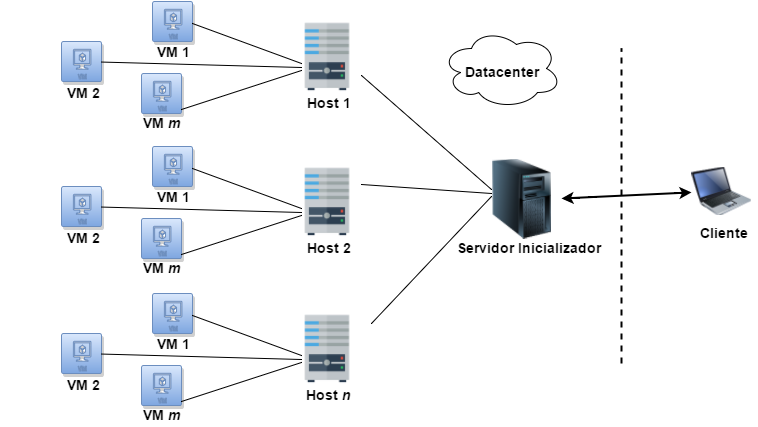
\includegraphics[scale=0.5]{media/cloud2}
	\caption{Propuesta de arquitectura en la nube, Fuente: Elaboraci'on propia. }
\end{figure}
%%%%%%%%
%%  IMAGEN
%%%


En la figura 1 se puede observar la arquitectura del centro de datos que se implementar'a en la investigaci'on, el cual est'a compuesto de los siguientes elementos:

\begin{itemize}
	\item \textbf{Servidor administrador:} Es el servidor que tendr'a el rol de front end en el centro de datos, teniendo una interacci'on directa con las peticiones de los usuarios, que son especificados en 'este documento como trabajos.
	El principal objetivo de 'este elemento es delegar los trabajos a las m'aquinas virtuales en los distintos hosts del centro de datos.
	\item \textbf{Host:} es el recurso de hardware que se tiene en el centro de datos. Una de las caracter'isticas de 'este elemento es que es finito.
	\item \textbf{M'aquinas Virtuales:} son instancias dentro de los host, tienen como objetivo resolver los trabajos que se les sea asignado.
\end{itemize}


\section*{Objetivos}
\addcontentsline{toc}{section}{Objetivos}


\subsection*{Objetivo general}
\addcontentsline{toc}{section}{Objetivo general}


Determinar y proponer un nuevo esquema que pueda resolver de manera eficiente el problema de la calendarizaci'on de un centro de datos y satisfacer las necesidades de un sistema ERP en la nube.


\subsection*{Objetivos espec'ificos}
\addcontentsline{toc}{section}{Objetivos espec'ificos}


\begin{itemize}
	\item Definir una arquitectura para un centro de datos en la nube con las necesidades de un sistema ERP.
	\item Realizar la simulaci'on en base a la arquitectura del centro de datos.
	\item Realizar e implementar diferentes esquemas de distribuci'on de trabajos, rescatando sus caracter'isticas principales.
	\item Reunir las caracter'isticas principales y proponer el nuevo esquema de distribuci'on.
	\item Aplicar el nuevo esquema de distribuci'on a las necesidades de un ERP.
	\item Comparar los resultados obtenidos del nuevo esquema propuesto y de los anteriores para determinar si hubo una mejora.
\end{itemize}


\newpage

\section*{Hip'otesis}
\addcontentsline{toc}{section}{Hip'otesis}

La modificaci'on de un esquema de distribuci'on mejorar'a el rendimiento de la calendarizaci'on para un sistema ERP en la nube.

Para realizar la verificaci'on de validez de la hip'otesis se usar'an:


\begin{itemize}
	\item \textbf{Pruebas de hardware y software:}
	\begin{itemize}
	\item \textbf{Prueba de desempe'no:} Validar el tiempo de respuesta para las tareas bajo condiciones normales y m'aximas.
	\item \textbf{Prueba de carga:} Verificar el tiempo de respuesta del sistema, bajo diferentes condiciones de carga. Se mide el tiempo de respuesta y otros requisitos sensibles al tiempo.
	\end{itemize}
	\item \textbf{Estad'isticas:} en base a los resultados que se obtendr'an en las pruebas de desempe'no y de carga, se va realizar comparaciones y posteriormente visualizarlas por medio de gr'aficas y tablas.
\end{itemize}

%% Los cap'itulos inician con \chapter{T'itulo}, estos aparecen numerados y
%% se incluyen en el 'indice general.
%%
%% Recuerda que aqu'i ya puedes escribir acentos como: 'a, 'e, 'i, etc.
%% La letra n con tilde es: 'n.

\chapter*{Propuesta y Justificaci\'on}
\addcontentsline{toc}{chapter}{Propuesta y Justificaci\'on}

Debido a la atenci'on que se tiene en la tecnolog'ia en la nube, los centros de datos han tomado un papel muy importante para los servicios empresariales.[2] Un centro de datos est'a compuesto por miles servidores virtuales ejecut'andose en una instancia de tiempo, alojando muchas tareas al mismo tiempo el centro de datos recibe miles de peticiones a esas tareas. Es aqu'i en donde la programaci'on de tareas tiene un rol demasiado importante para el c'omputo en la nube porque influye en el rendimiento del mismo.[1] 

El problema de la calendarizaci'on pertenece a los algoritmos NP-Dif'icil, lo cual tiene un amplio rango de soluciones posibles y se toma mucho m'as tiempo de encontrar una respuesta 'optima ya que no existe un m'etodo para resolver estas inc'ognitas. Sin embargo es posible estar cerca de la mejor soluci'on contemplando algunos entornos.[2]

En esta investigaci'on se propondr'a una mejora a un algoritmo de calendarizaci'on para el caso de estudio de un sistema ERP en la nube, contemplando sus posibles escenarios y peticiones heterog'eneas.De esta manera se podr'a contar con un esquema de distribuci'on de trabajos que satisfaga las necesidades de un sistema ERP,mejorando el tiempo de respuesta y aprovechando los recursos.Con beneficios a los proveedores de servicios (SaaS) de sistemas ERP.
%% Los cap'itulos inician con \chapter{T'itulo}, estos aparecen numerados y
%% se incluyen en el 'indice general.
%%
%% Recuerda que aqu'i ya puedes escribir acentos como: 'a, 'e, 'i, etc.
%% La letra n con tilde es: 'n.

\chapter*{Objetivos}
\addcontentsline{toc}{chapter}{Objetivos}

\section*{Objetivo general}
\addcontentsline{toc}{section}{Objetivo general}


Determinar y proponer un nuevo esquema que pueda resolver de una manera eficiente el problema de la calendarizaci'on de un centro de datos y satisfacer las necesidades de un sistema ERP en la nube.


\section*{Objetivos espec'ificos}
\addcontentsline{toc}{section}{Objetivos espec'ificos}


\begin{itemize}
\item Definir una arquitectura para un centro de datos en la nube con las necesidades de un sistema ERP.
\item Realizar la simulaci'on en base a la arquitectura del centro de datos.
\item Realizar e implementar diferentes esquemas de distribuci'on de trabajos, rescatando sus caracter'isticas principales.
\item Reunir las caracter'isticas principales y proponer el nuevo esquema de distribuci'on.
\item Aplicar el nuevo esquema de distribuci'on a las necesidades de un ERP.
\item Comparar los resultados obtenidos del nuevo esquema propuesto y de los anteriores para determinar si hubo una mejora.
\end{itemize}

%% Los cap'itulos inician con \chapter{T'itulo}, estos aparecen numerados y
%% se incluyen en el 'indice general.
%%
%% Recuerda que aqu'i ya puedes escribir acentos como: 'a, 'e, 'i, etc.
%% La letra n con tilde es: 'n.

\chapter*{Hip\'otesis}
\addcontentsline{toc}{chapter}{Hip\'otesis}


\begin{itemize}
\item La modificaci'on de un esquema de distribuci'on mejorar'a el rendimiento de un sistema ERP en la nube.
\end{itemize}


\chapter*{Metodolog\'ia}
\addcontentsline{toc}{chapter}{Metodolog\'ia}

\begin{itemize}
\item \textbf{Simular:} Se implementar'a a manera de simulaci'on un centro de datos con un entorno en la nube, las m'aquinas virtuales y el servidor inicializador que lo conforman.
\item \textbf{Implementar:} En el centro de datos se desarrollar'an los algoritmos de calendarizaci'on que se mencionan con antelaci'on.
\item \textbf{Evaluar:} Se simular'a el comportamiento de las peticiones de un sistema contemplando los distintos escenarios del ERP y consumiendo el servicio en la nube (SaaS), para conocer el rendimiento en tiempo de ejecuci'on de los algoritmos.
\item \textbf{Mejorar:} Se propondr'a una mejora a algún algoritmo de acuerdo a las necesidades y comportamiento de un sistema ERP en la nube.
\item \textbf{Comparar:} Se realizar'a una comparativa de tiempo de ejecuci'on entre la versi'on mejorada y la original para el caso de estudio de un sistema ERP.
\end{itemize}
%%%% Los cap'itulos inician con \chapter{T'itulo}, estos aparecen numerados y
%% se incluyen en el 'indice general.
%%
%% Recuerda que aqu'i ya puedes escribir acentos como: 'a, 'e, 'i, etc.
%% La letra n con tilde es: 'n.

\chapter*{Metodolog\'ia}
\addcontentsline{toc}{chapter}{Metodolog\'ia}
\chapter*{Plan de trabajo}
\addcontentsline{toc}{chapter}{Plan de trabajo}
\centering
\hspace*{-1.8cm}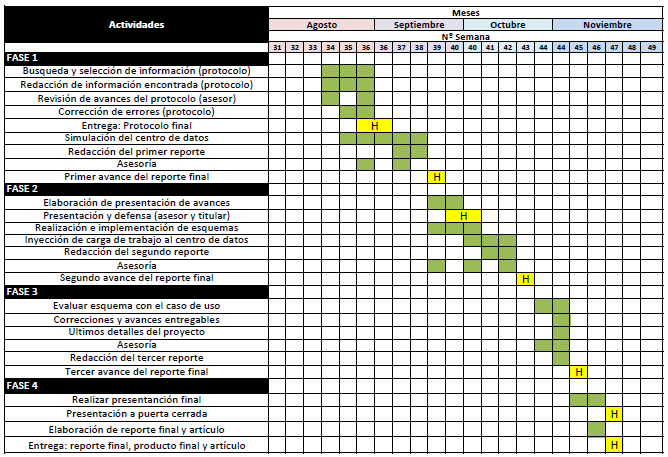
\includegraphics[]{media/trabajo}

\addcontentsline{toc}{chapter}{Bibliografia}
\bibliographystyle{plain}
%\include{conclu}

\appendix
%% Cap'itulos incluidos despues del comando \appendix aparecen como ap'endices
%% de la tesis.
∞\include{apendiceA}
%\include{apendiceB}
%\include{apendiceC}

%% Incluir la bibliograf'ia. Mirar el archivo "biblio.bib" para m'as detales
%% y un ejemplo.
\bibliography{biblio}

\end{document}
